\chapter{Analisi Esplorativa del Dataset}
\label{chap:chap3}

In questo capitolo viene presentata l'analisi esplorativa dei dati (EDA) condotta sul dataset MovieLens 100k, con l'obiettivo di comprendere la struttura, le caratteristiche e le criticità dei dati utilizzati per la sperimentazione dei sistemi di raccomandazione. L'analisi è stata svolta tramite lo script Python \texttt{eda\_movielens100k.py}, che genera automaticamente tutti i plot e le statistiche descritte di seguito.

\section{Descrizione del Dataset}
Il dataset MovieLens 100k contiene 100.000 valutazioni espresse da 943 utenti su 1682 film. Ogni valutazione è un intero da 1 a 5. Sono inoltre disponibili informazioni anagrafiche sugli utenti (età, genere, occupazione) e sui film (titolo, data di uscita, generi associati).

\subsection{Filtraggio e Preprocessing}
Per ottenere una base dati densa e affidabile, durante l'analisi esplorativa sono stati applicati filtraggi sui dati grezzi:
\begin{itemize}
    \item Sono stati mantenuti solo gli utenti con almeno 150 valutazioni.
    \item Sono stati mantenuti solo i film con almeno 150 valutazioni.
\end{itemize}
Questo ha ridotto il dataset a 24669 valutazioni, 230 utenti e 203 film, rendendo più affidabile l'analisi dei cluster.   

\begin{figure}[H]
  \centering
  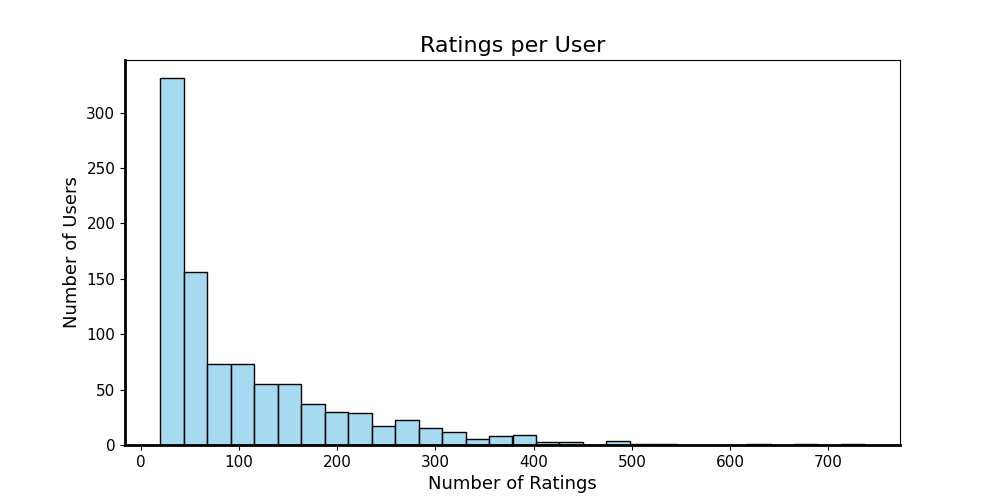
\includegraphics[width=0.48\textwidth]{../output/eda/before_cut/before_ratings_per_user_hist.png}
  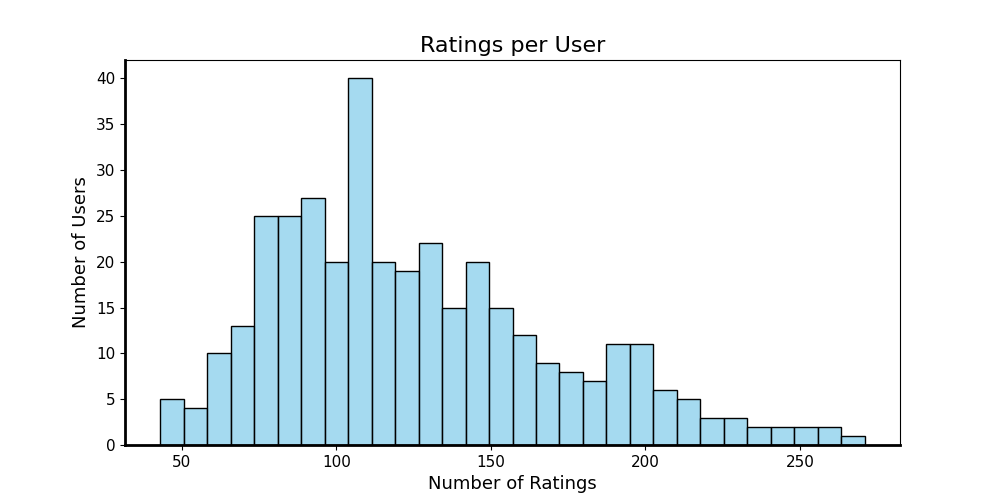
\includegraphics[width=0.48\textwidth]{../output/eda/after_cut/after_ratings_per_user_hist.png}
  \caption{Distribuzione del numero di valutazioni per utente, prima e dopo il filtraggio.}
\end{figure}

\begin{figure}[H]
  \centering
  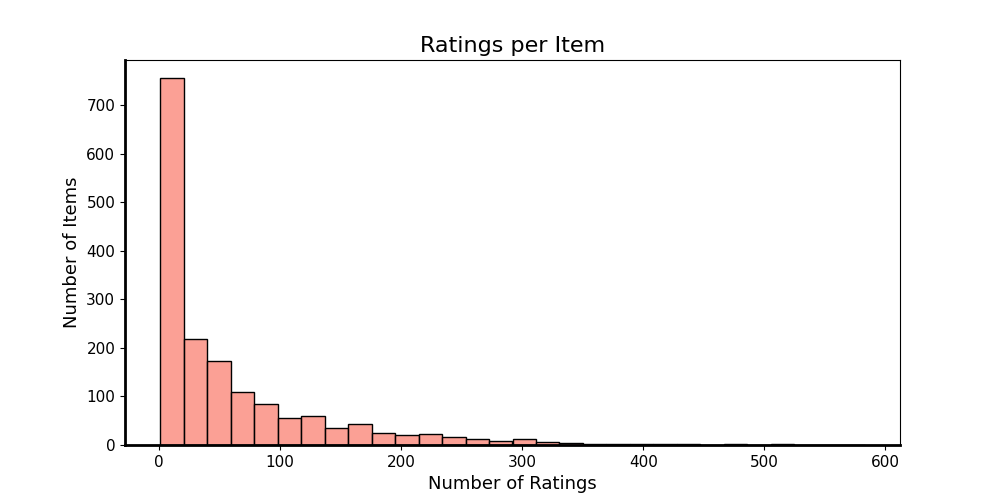
\includegraphics[width=0.48\textwidth]{../output/eda/before_cut/before_ratings_per_item_hist.png}
  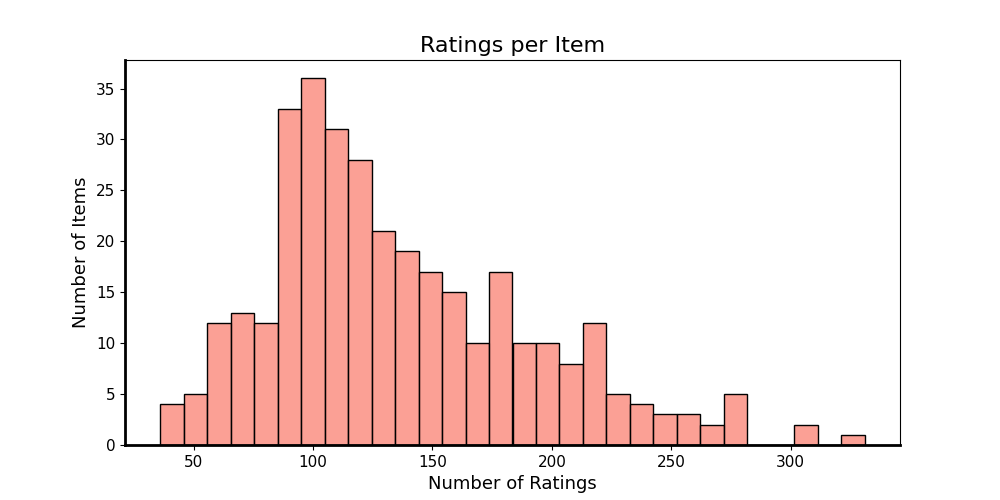
\includegraphics[width=0.48\textwidth]{../output/eda/after_cut/after_ratings_per_item_hist.png}
  \caption{Distribuzione del numero di valutazioni per film, prima e dopo il filtraggio.}
\end{figure}

\section{Distribuzione delle Valutazioni}
La distribuzione delle valutazioni mostra una forte asimmetria verso i valori alti. Questo bias positivo può influenzare le metriche di errore e la qualità delle raccomandazioni.

\begin{figure}[H]
    \centering
    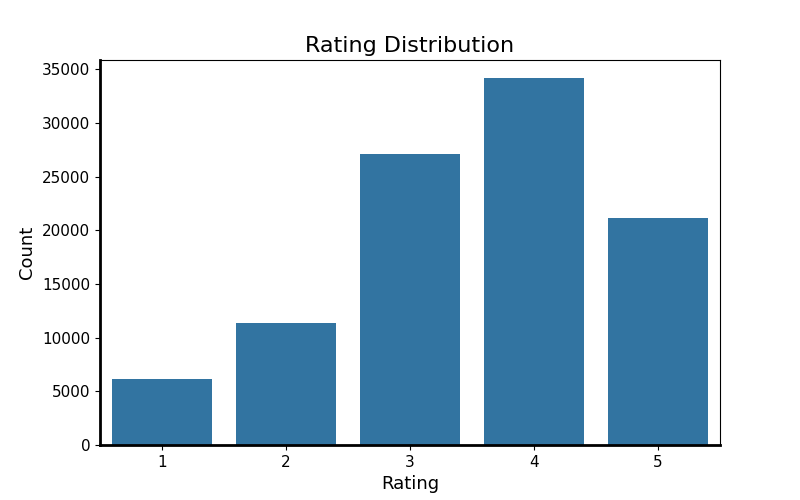
\includegraphics[width=0.6\textwidth]{../output/eda/before_cut/before_rating_distribution.png}
    \caption{Distribuzione delle valutazioni (prima del filtraggio).}
\end{figure}

\begin{figure}[H]
    \centering
    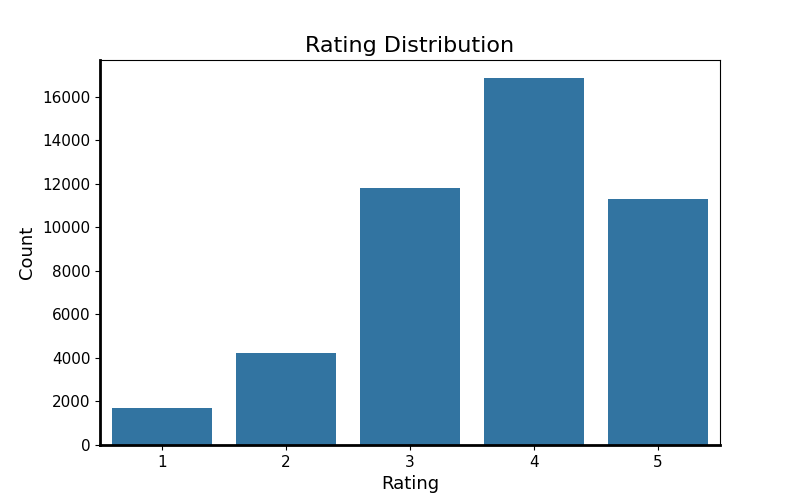
\includegraphics[width=0.6\textwidth]{../output/eda/after_cut/after_rating_distribution.png}
    \caption{Distribuzione delle valutazioni (dopo il filtraggio).}
\end{figure}

\subsection{Valutazioni per utente e per film}
I boxplot delle valutazioni per utente e per film evidenziano la presenza di outlier e la variabilità tra utenti e tra film.

Si può osservare come il filtraggio ha eliminato i valori più alti, lasciando solo i valori più centrali, e quindi i valori più rappresentativi.

\begin{figure}[H]
    \centering
    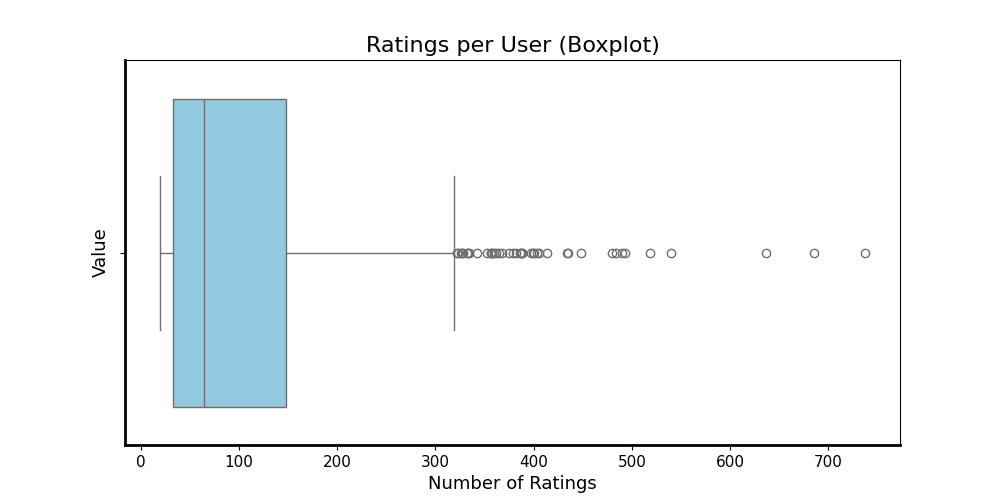
\includegraphics[width=0.48\textwidth]{../output/eda/before_cut/before_ratings_per_user_box.png}
    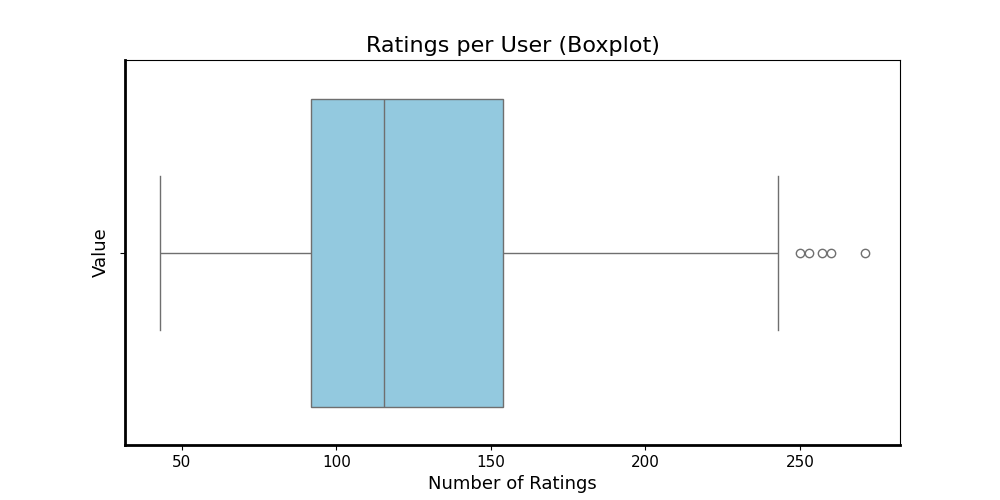
\includegraphics[width=0.48\textwidth]{../output/eda/after_cut/after_ratings_per_user_box.png}
    \caption{Boxplot del numero di valutazioni per utente, prima e dopo il filtraggio.}
\end{figure}

\begin{figure}[H]
    \centering
    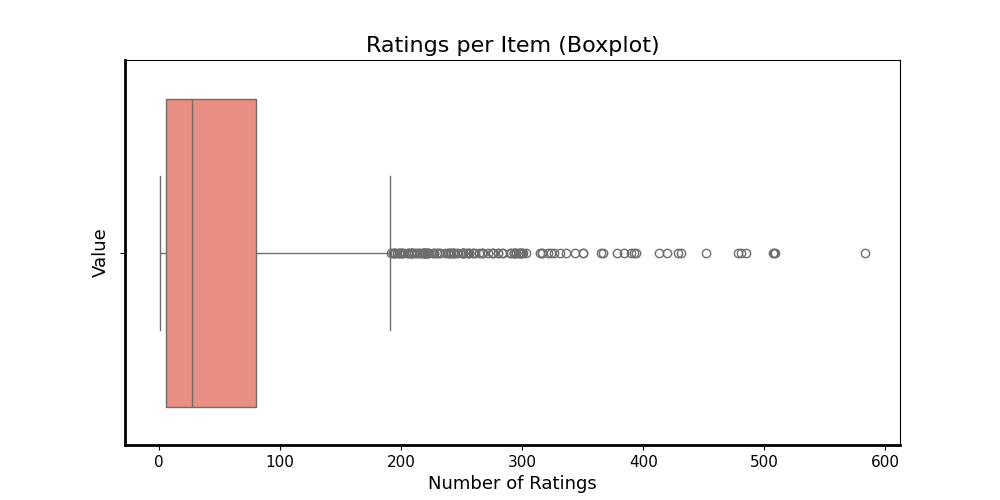
\includegraphics[width=0.48\textwidth]{../output/eda/before_cut/before_ratings_per_item_box.png}
    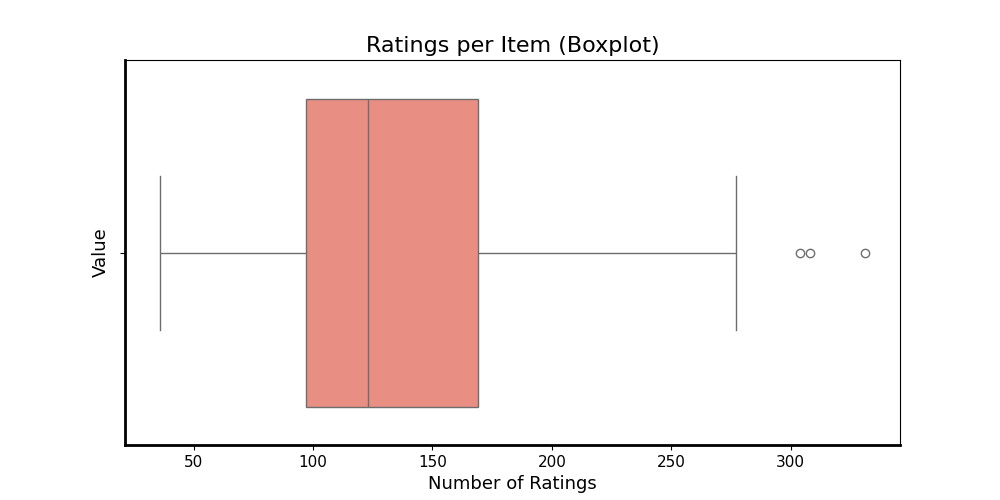
\includegraphics[width=0.48\textwidth]{../output/eda/after_cut/after_ratings_per_item_box.png}
    \caption{Boxplot del numero di valutazioni per film, prima e dopo il filtraggio.}
\end{figure}

\section{Sparsità della Matrice Utente-Item}
La matrice delle valutazioni è estremamente sparsa: anche dopo il filtraggio, la maggior parte delle possibili coppie utente-film non ha una valutazione. Questo può comportare problemi nell'analisi dei dati e nella generazione di raccomandazioni.

\begin{figure}[H]
    \centering
    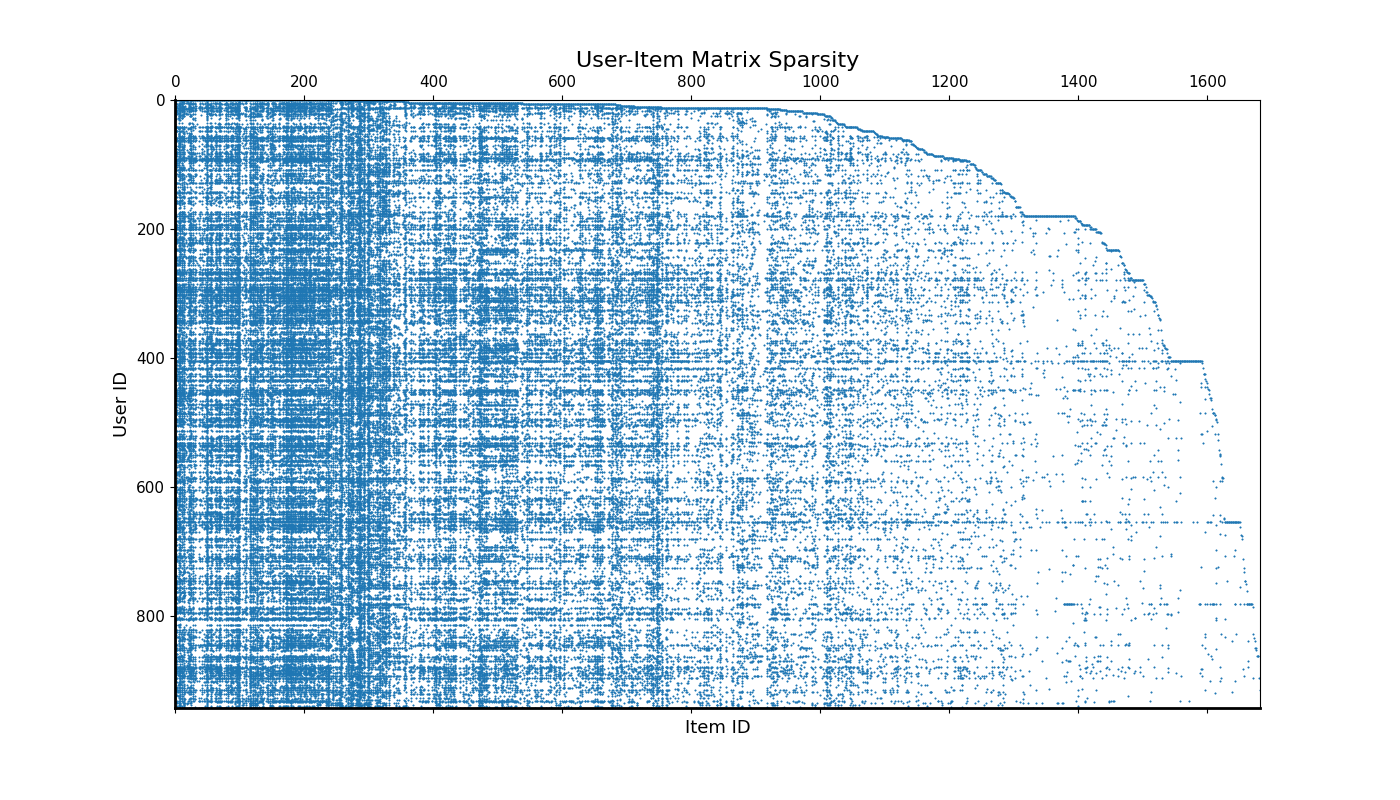
\includegraphics[width=0.48\textwidth]{../output/eda/before_cut/before_sparsity_matrix.png}
    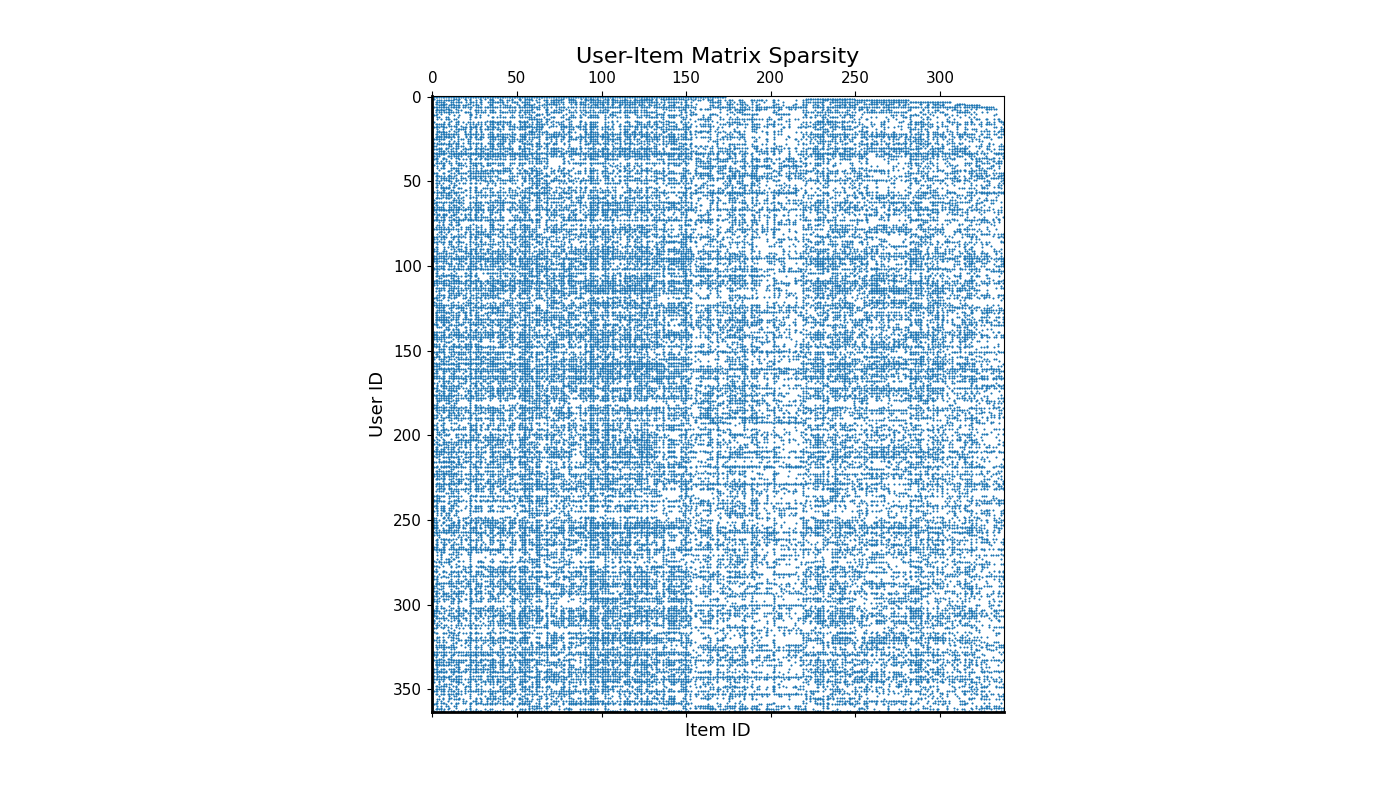
\includegraphics[width=0.48\textwidth]{../output/eda/after_cut/after_sparsity_matrix.png}
    \caption{Visualizzazione della matrice utente-item, prima e dopo il filtraggio.}
\end{figure}

\subsection{Correlazioni tra Utenti e tra Film}
Sono state calcolate le matrici di correlazione (Pearson) tra utenti e tra film, su un campione di 50 utenti/film per leggibilità. Come si può osservare, non sembra esserci una correlazione tra utenti e film evidente.

\begin{figure}[H]
    \centering
    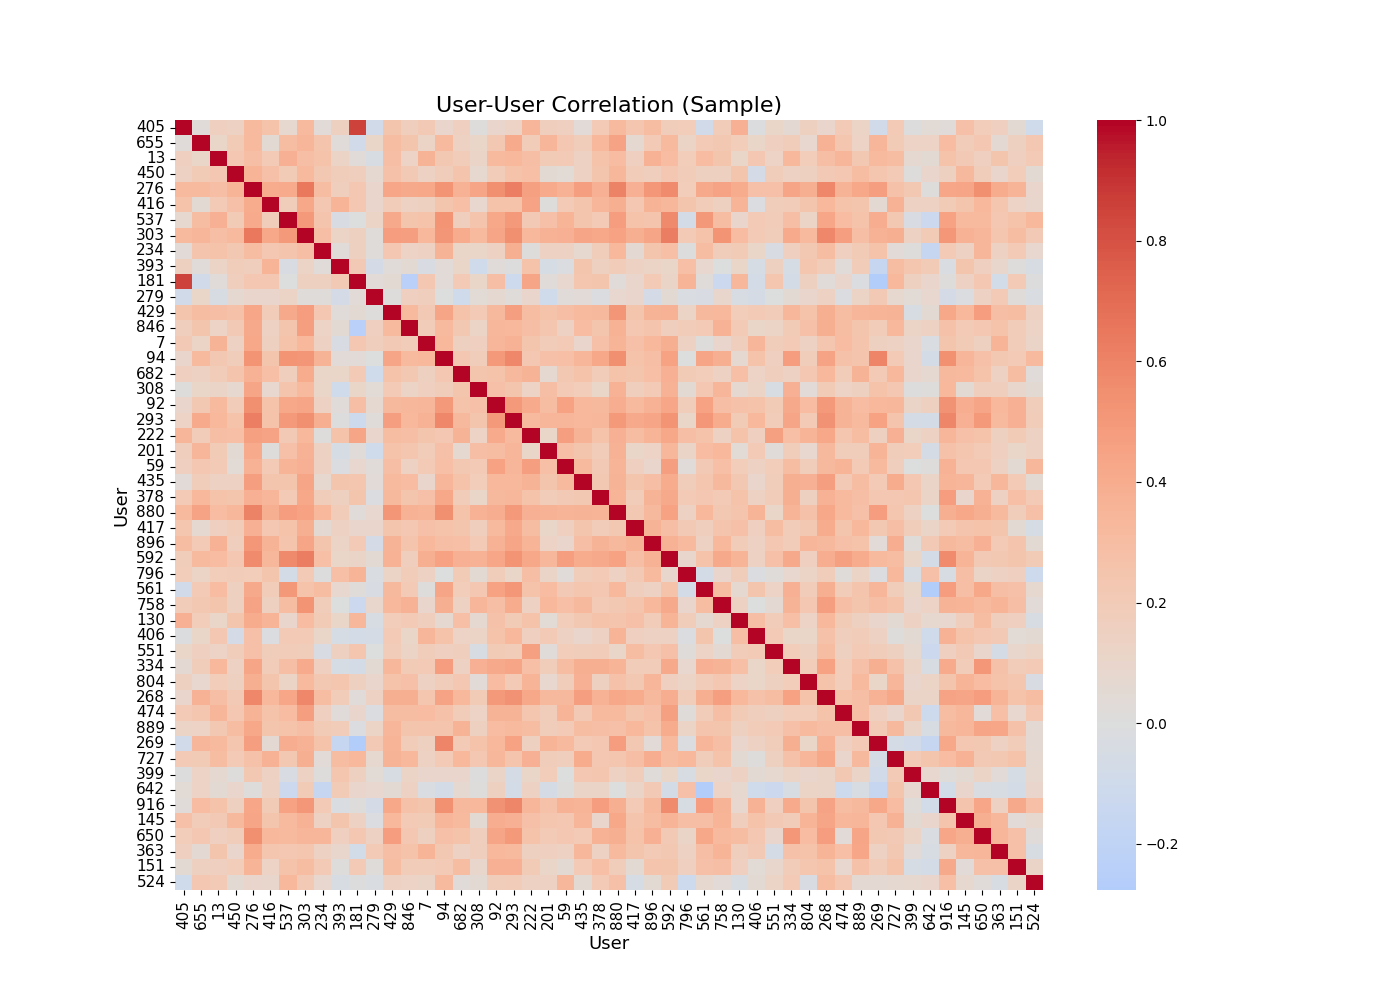
\includegraphics[width=0.48\textwidth]{../output/eda/before_cut/before_user_correlation_heatmap.png}
    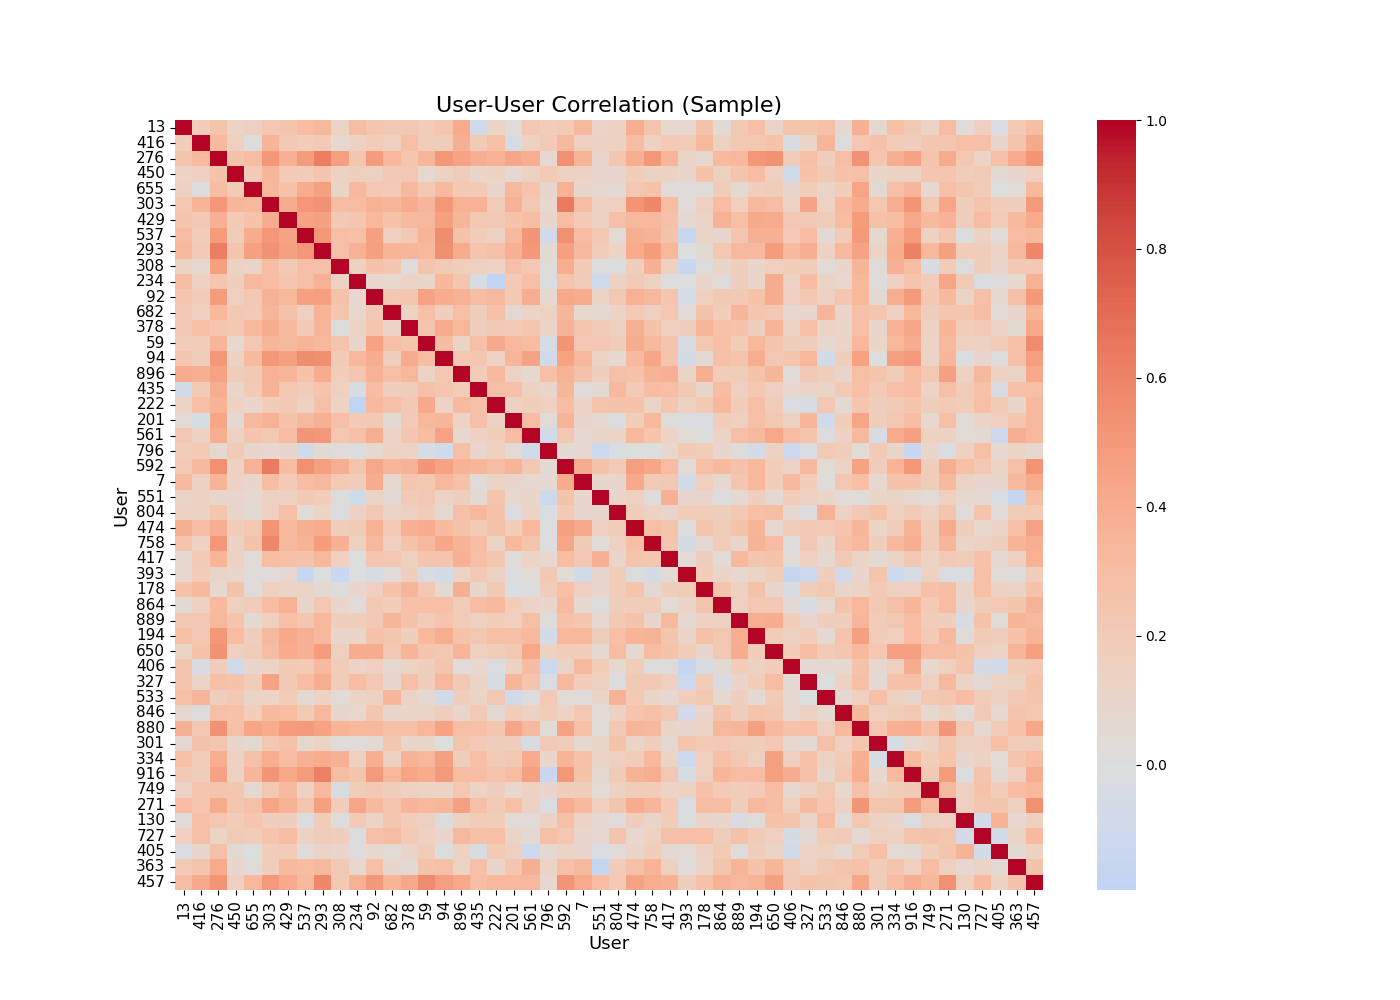
\includegraphics[width=0.48\textwidth]{../output/eda/after_cut/after_user_correlation_heatmap.png}
    \caption{Heatmap delle correlazioni tra utenti, prima e dopo il filtraggio.}
\end{figure}

\begin{figure}[H]
    \centering
    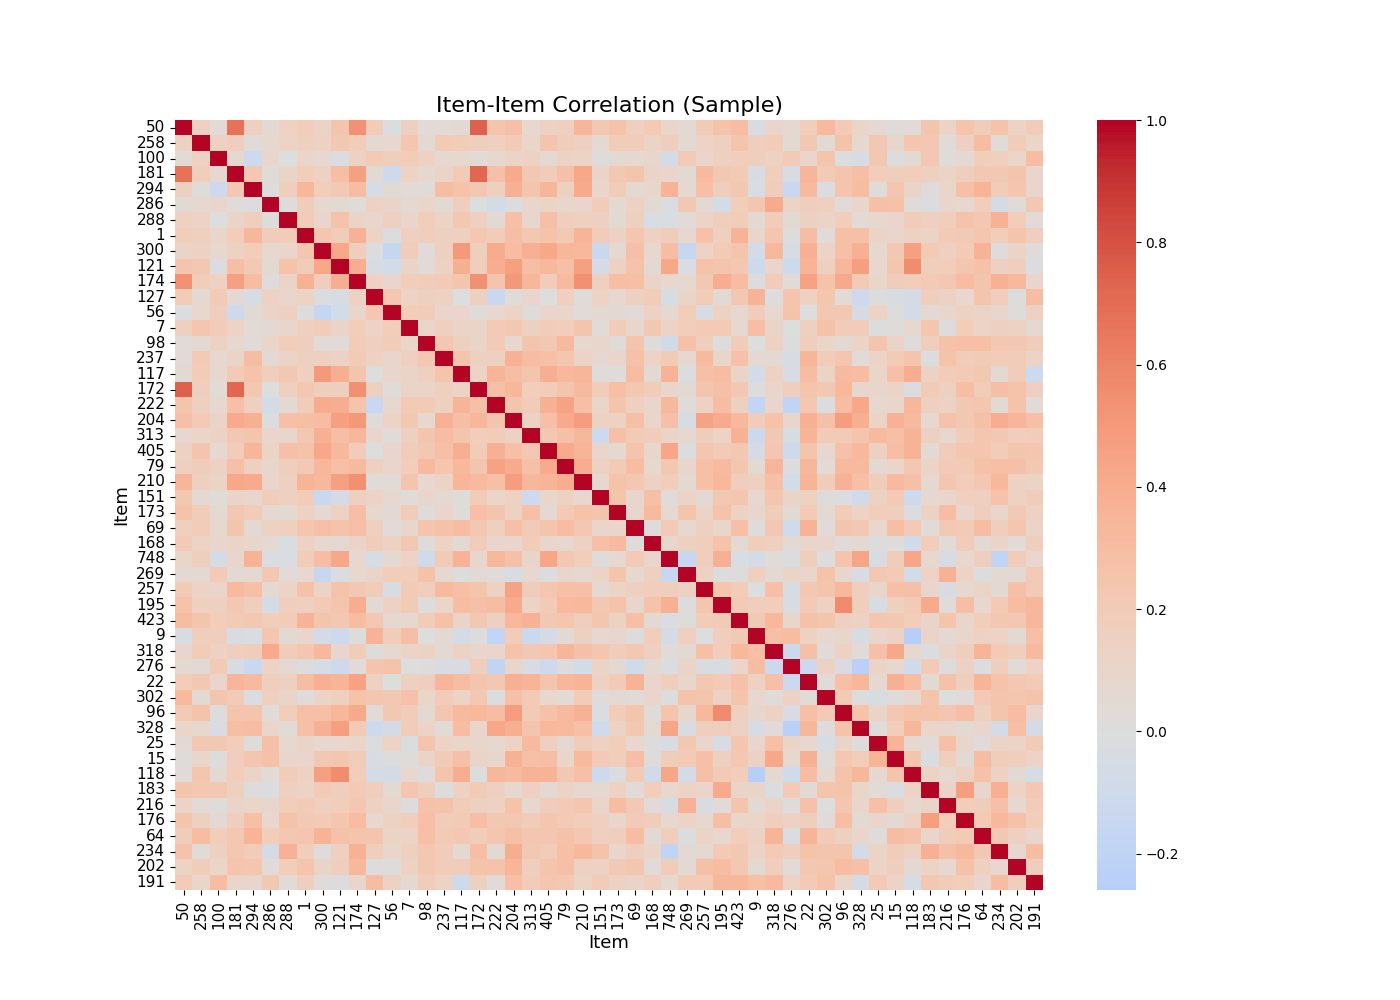
\includegraphics[width=0.48\textwidth]{../output/eda/before_cut/before_item_correlation_heatmap.png}
    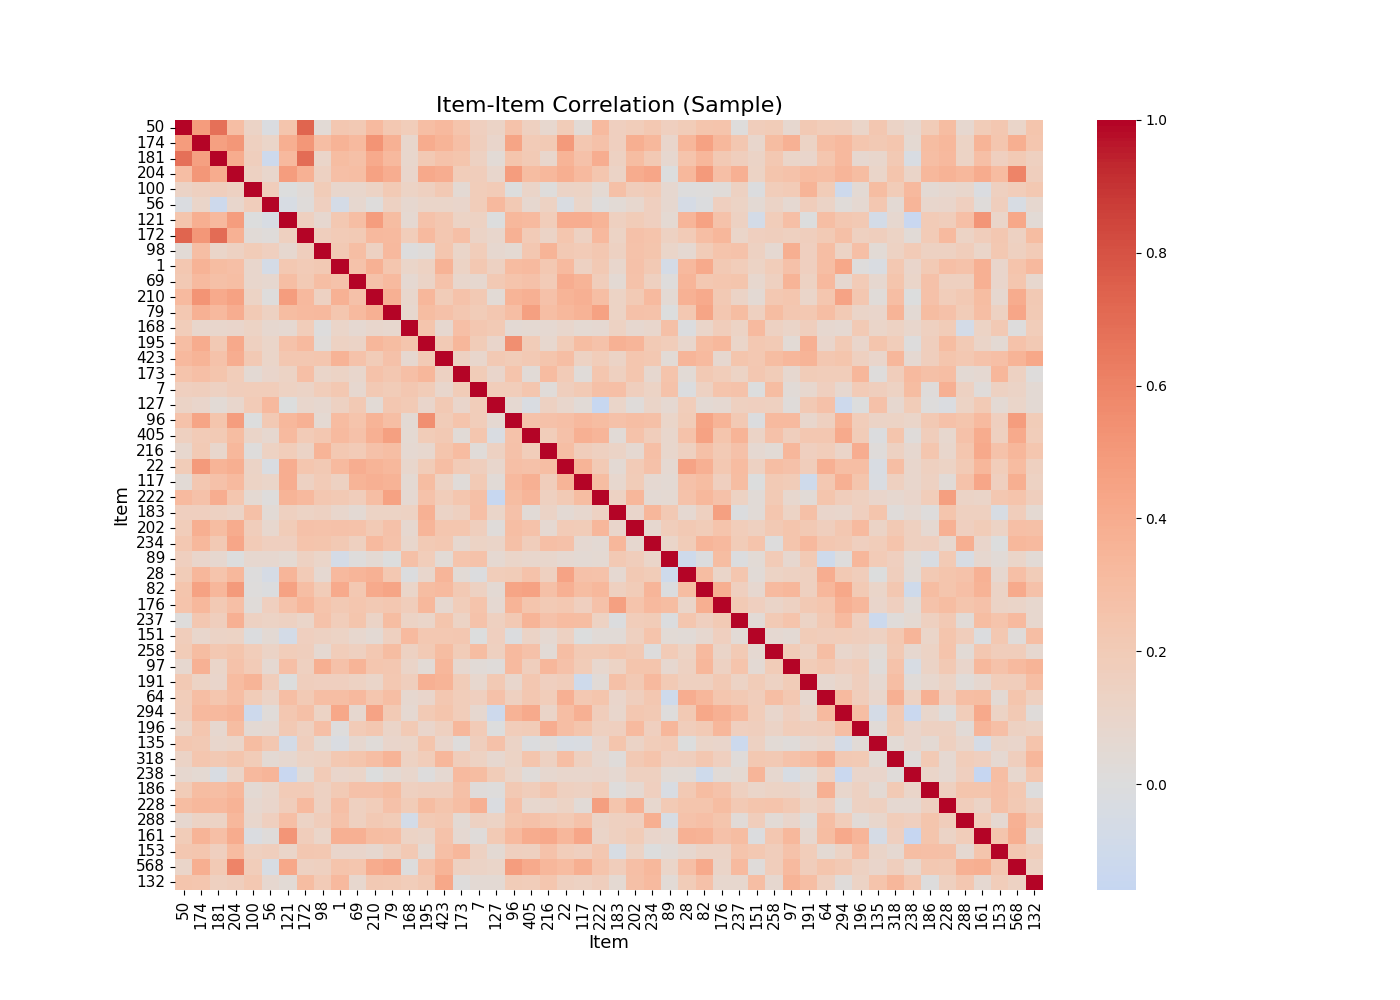
\includegraphics[width=0.48\textwidth]{../output/eda/after_cut/after_item_correlation_heatmap.png}
    \caption{Heatmap delle correlazioni tra film, prima e dopo il filtraggio.}
\end{figure}

\subsection{Analisi dei Generi}
L'analisi dei generi mostra una forte predominanza di alcuni generi (drama, comedy, action), mentre altri sono molto meno rappresentati. Questo può influenzare la varietà delle raccomandazioni.

\begin{figure}[H]
    \centering
    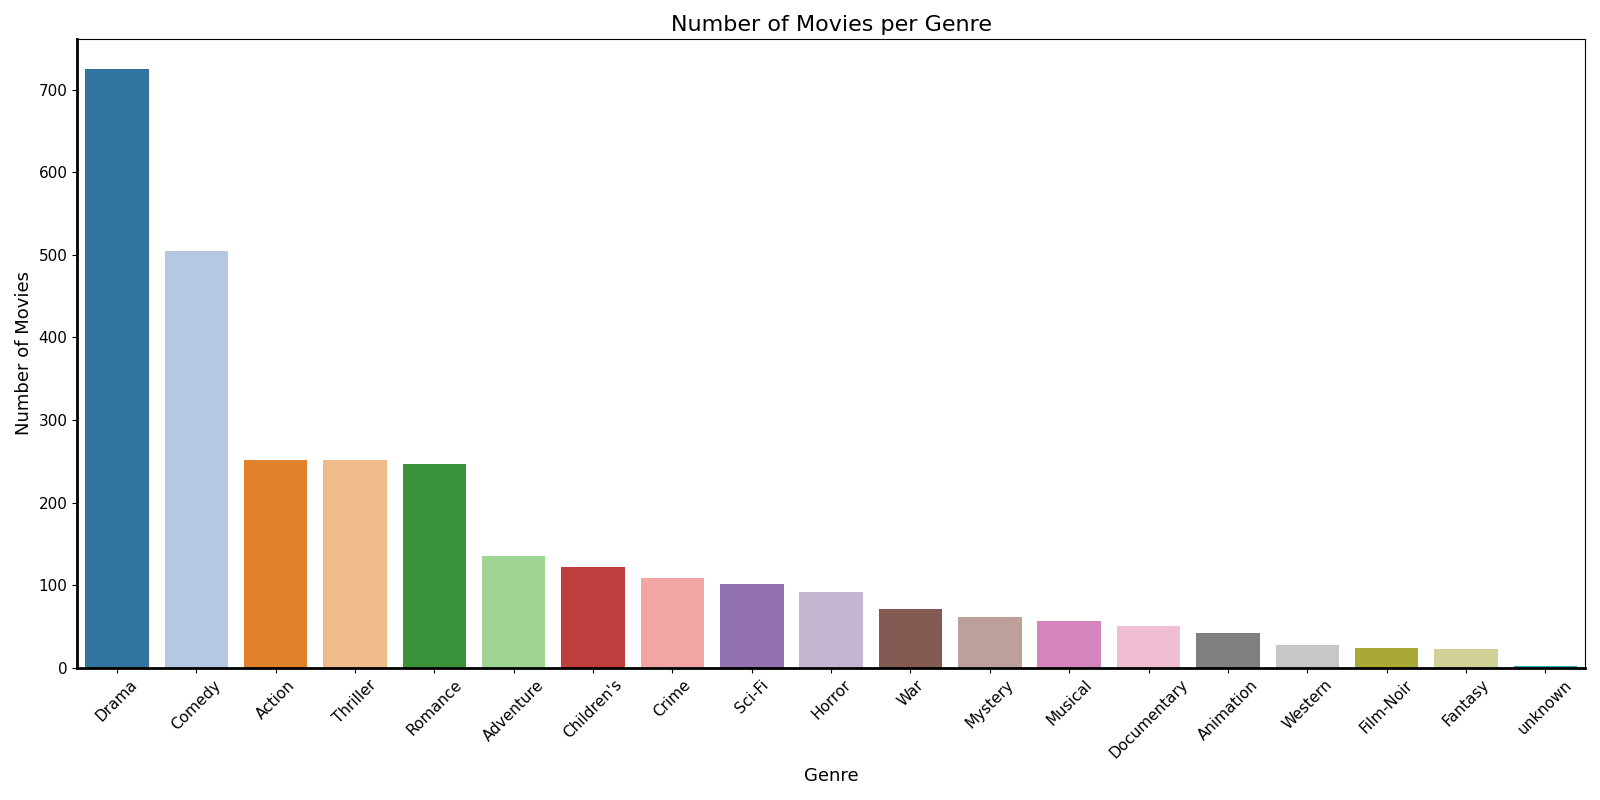
\includegraphics[width=0.8\textwidth]{../output/eda/before_cut/before_movies_per_genre.png}
    \caption{Numero di film per genere (prima del filtraggio).}
\end{figure}

\section{MovieLens 1M}

Sebbene il sistema realizzato supporta l'utilizzo del dataset MovieLens 1M, è stato scelto di utilizzare il dataset MovieLens 100k per la sperimentazione, in quanto più compatto e più facile da gestire. L'analisi di quest'ultimo può essere considerata come un'estensione futura di questo lavoro.
